%%%%%%%%%%%%%%%%%%%%%%%%%%%%%%%%%%%%%%%%%
% Beamer Presentation
% LaTeX Template
% Version 1.0 (10/11/12)
%
% This template has been downloaded from:
% http://www.LaTeXTemplates.com
%
% License:
% CC BY-NC-SA 3.0 (http://creativecommons.org/licenses/by-nc-sa/3.0/)
%
%%%%%%%%%%%%%%%%%%%%%%%%%%%%%%%%%%%%%%%%%

%----------------------------------------------------------------------------------------
%	PACKAGES AND THEMES
%----------------------------------------------------------------------------------------

\documentclass{beamer}

\mode<presentation> {

% The Beamer class comes with a number of default slide themes
% which change the colors and layouts of slides. Below this is a list
% of all the themes, uncomment each in turn to see what they look like.

%\usetheme{default}
%\usetheme{AnnArbor}
%\usetheme{Antibes}
%\usetheme{Bergen}
%\usetheme{Berkeley}
%\usetheme{Berlin}
%\usetheme{Boadilla}
%\usetheme{CambridgeUS}
%\usetheme{Copenhagen}
%\usetheme{Darmstadt}
%\usetheme{Dresden}
%\usetheme{Frankfurt}
%\usetheme{Goettingen}
%\usetheme{Hannover}
%\usetheme{Ilmenau}
%\usetheme{JuanLesPins}
%\usetheme{Luebeck}
\usetheme{Madrid}
%\usetheme{Malmoe}
%\usetheme{Marburg}
%\usetheme{Montpellier}
%\usetheme{PaloAlto}
%\usetheme{Pittsburgh}
%\usetheme{Rochester}
%\usetheme{Singapore}
%\usetheme{Szeged}
%\usetheme{Warsaw}

% As well as themes, the Beamer class has a number of color themes
% for any slide theme. Uncomment each of these in turn to see how it
% changes the colors of your current slide theme.

%\usecolortheme{albatross}
%\usecolortheme{beaver}
%\usecolortheme{beetle}
%\usecolortheme{crane}
%\usecolortheme{dolphin}
%\usecolortheme{dove}
%\usecolortheme{fly}
%\usecolortheme{lily}
%\usecolortheme{orchid}
%\usecolortheme{rose}
%\usecolortheme{seagull}
%\usecolortheme{seahorse}
%\usecolortheme{whale}
%\usecolortheme{wolverine}

%\setbeamertemplate{footline} % To remove the footer line in all slides uncomment this line
%\setbeamertemplate{footline}[page number] % To replace the footer line in all slides with a simple slide count uncomment this line

%\setbeamertemplate{navigation symbols}{} % To remove the navigation symbols from the bottom of all slides uncomment this line
}

\usepackage{graphicx} % Allows including images
\usepackage{booktabs} % Allows the use of \toprule, \midrule and \bottomrule in tables
\usepackage[utf8]{inputenc}
% \usepackage[font={small,it}]{caption}

\DeclareMathOperator*{\argmax}{arg\,max}

%----------------------------------------------------------------------------------------
%	TITLE PAGE
%----------------------------------------------------------------------------------------

\title[Neural Networks and SMT]{Neural Networks and Statistical Machine Translation} % The short title appears at the bottom of every slide, the full title is only on the title page

\author{Gaurav Kumar} % Your name
\institute[CLSP] % Your institution as it will appear on the bottom of every slide, may be shorthand to save space
{
Center for Language and Speech Processing \\ % Your institution for the title page
Johns Hopkins University\\
\medskip
\textit{gkumar@cs.jhu.edu} % Your email address
}
\date{\today} % Date, can be changed to a custom date

\begin{document}

\begin{frame}
\titlepage % Print the title page as the first slide
\end{frame}

\begin{frame}
\frametitle{Overview} % Table of contents slide, comment this block out to remove it
\tableofcontents % Throughout your presentation, if you choose to use \section{} and \subsection{} commands, these will automatically be printed on this slide as an overview of your presentation
\end{frame}


%----------------------------------------------------------------------------------------
%	PRESENTATION SLIDES
%----------------------------------------------------------------------------------------

%------------------------------------------------
\section{Overview of Machine Translation} % Sections can be created in order to organize your presentation into discrete blocks, all sections and subsections are automatically printed in the table of contents as an overview of the talk
%------------------------------------------------

\begin{frame}
\frametitle{Speech Translation}
Given a source (foreign) sentence $f$, we want to find the target (english) sentence $e$
\begin{align*}
\argmax_e p(e|f) &= \argmax_e p(f|e) \times p(e) \;\;\;\;\; \intertext{Using the Bayes rule} 
\intertext{Also,}
p(f|e) & = \sum_a p(a,f|e)
\end{align*}
% \begin{frame}
\end{frame}
% \end{frame}
% \begin{block}{Speech Translation}
% To translate speech in one language (eg. Arabic) to text/speech in another language (eg. English)
% \end{block} 
% This generally involves :
% \begin{itemize}
% 	\item Get automatic transcripts from speech (ASR)
% 	\item Get translations of these automatic transcripts (SMT)
% 	\item Convert translations to speech (TTS)
% \end{itemize}
% \begin{figure}
% 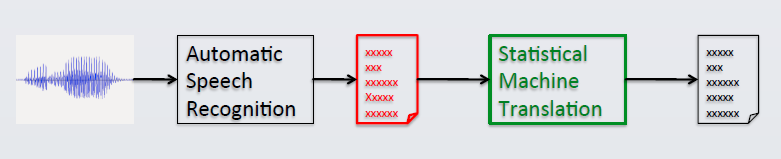
\includegraphics[width=0.8\linewidth]{pipeline.png}
% \end{figure}


\end{document}

%------------------------------------------------

\begin{frame}
\frametitle{The Egyptian Arabic Callhome Corpus}
\begin{itemize}
	\item Callhome Egyptian Arabic Speech/Transcripts (ECA-96 : train, dev, test)
	\item 1997 HUB5 Arabic Evaluation (97-eval-H5)
	\item Callhome Egyptian Arabic Speech/Transcripts Supplement (ECA-supplement)
\end{itemize}

\begin{table}
	\begin{center}
 	\begin{tabular}{| l | c | r | r | c |}
 	\hline
   	\textbf{Partition} & \textbf{\# Conv } & \textbf{\# Utt's } & \textbf{\# Words} & \textbf{Words/Utt} \\ \hline
   	ECA-96 (train) & 80 &20,861 & 139,035 & 6.66\\
   	\hline
   	ECA-96 (dev) & 20 & 6,415 & 34,543 & 5.38\\
   	\hline
   	ECA-96 (test) & 20 & 3,044 & 16,500 & 5.42\\
   	\hline
   	97-eval-H5 & 20 & 2,800 & 18,845 & 6.73\\
   	\hline
   	ECA-supplement & 20 & 2,772 & 18,039 & 6.51\\
   	\hline
 	\end{tabular}
 	\caption{Partition statistics for the Callhome Egyptian Arabic corpus, supplements and evaluation datasets.}
 	\label{tab:partition-stat}
 	\end{center}
\end{table}

\end{frame}

%------------------------------------------------

\begin{frame}
\frametitle{The Egyptian Arabic Callhome Corpus : Translations}
We currently use translations of the Callhome Egyptian Arabic Corpus generated at JHU \footnote{\tiny{Kumar et al., \textit{Speech Translation with the Callhome Egyptian Arabic Corpus}, IEEE SLT, 2014 (submitted)}}. 
\textbf{Four} alternative translations were created for each utterance in the corpus.
\begin{itemize}
\item Collected via Amazon's Mechanical Turk platform.
\item Translations by native speakers of the source language.
\item Quality control and post editing done.
\end{itemize}

\begin{table}
\begin{center}
\begin{tabular}{| l | c | c | c |}
  \hline 
  \textbf{Partition} & \textbf{\# Utt's } & \textbf{\# Words} & \textbf{Words/Utt} \\ \hline
  ECA-96 (train) & 86,313 & 713,549 & 8.27\\
  \hline
  ECA-96 (dev) & 25,769 & 186,400 & 7.23\\
  \hline
  ECA-96 (test) & 12,212 & 85,182 & 6.98\\
  \hline
  97-eval-H5 & 11,248 & 91,647 & 8.15\\
  \hline
  ECA-supplement & 11,126 & 87,489 & 7.86\\
  \hline
\end{tabular}
\caption{Reference (English) translation statistics for the Egyptian-Arabic Callhome corpus.}
%\vspace*{-18pt}
\label{tab:trans-results}
\end{center}
\end{table}

\end{frame}

%------------------------------------------------

\begin{frame}
\frametitle{The Egyptian Arabic Callhome Corpus : Translations}
\begin{itemize}
	\item Inter-translator agreement is low.
	\item This is typical for human translations of informal speech/text.
	\item Diversity in translations required to compensate for possibility of multiple valid answers automatic SMT evaluation.
\end{itemize}

\begin{table}
\begin{center}
\begin{tabular}{| l | c |}
  \hline 
  \textbf{Partition} & \textbf{Crossfold BLEU} \\ \hline
  ECA-96 (train) & 40.09\%\\
  \hline
  ECA-96 (dev) & 35.64\%\\
  \hline
  ECA-96 (test) & 35.86\%\\
  \hline
  97-eval-H5 & 35.81\%\\
  \hline
  ECA-supplement & 37.15\%\\
  \hline
\end{tabular}
\caption{Crossfold (hold-1, against-3) average BLEU per partition of the Callhome Egyptian Arabic corpus, supplements and evaluation datasets.}
%\vspace*{-18pt}
\label{tab:cross-bleu}
\end{center}
\end{table}

\end{frame}

%------------------------------------------------

\begin{frame}
\frametitle{The Egyptian Arabic Callhome Corpus : Translations}
\begin{table}
\begin{center}
\begin{tabular}{| l | p{2.5in} |}
  \hline 
  \textbf{Source} & mA Antw mbtrdw\$ ElY Altlyfwn ybqY\cr
  \textbf{Translation 1} & you do n't reply to the phone\cr
  \textbf{Translation 2} & so you do n't answer the phone then\cr
  \textbf{Translation 3} & you do n't answer the phone it seems\cr
  \textbf{Translation 4} & because you do n't answer the call then\cr
  \hline
  \textbf{Source} & mSEbAn Elyh nfsh kmAn\cr
  \textbf{Translation 1} & he feels hard for himself too\cr
  \textbf{Translation 2} & he feel bad about himself\cr
  \textbf{Translation 3} & he feels sorry for himself too\cr
  \textbf{Translation 4} & i feel sorrow about his condition too\cr
  \hline
\end{tabular}
\caption{A sample of the translations for the Egyptian-Arabic Callhome Corpus. The translations are 
lower-cased, tokenized and punctuation has been normalized.}
%\vspace*{-18pt}
\label{tab:trans-sample}
\end{center}
\end{table}
\end{frame}

%------------------------------------------------

\begin{frame}
\frametitle{The ASR system}
\begin{itemize}
\item The ASR system is built using Kaldi @ JHU
\item Training data for acoustic modeling : $\sim$ 16 hours 
\item Automated evaluation using the NIST sclite scoring tool
\item This is work in progress, more data ($\sim$ 30 hours) recently available through LDC (+ $\sim$ 100 hours from GALE)
\end{itemize}
\begin{table}
\begin{center}
\begin{tabular}{| l | c |}
  \hline 
  \textbf{ASR Model} & \textbf{WER} \\ \hline
  Triphone + SAT (train) & 57.98\%\\
  \hline
  + SGMM (dev) & 52.74\%\\
  \hline
  + DNN (test) & 51.80\%\\
  \hline
\end{tabular}
\caption{Word error rates (WER) for ASR models}
%\vspace*{-18pt}
\label{tab:cross-bleu}
\end{center}
\end{table} 
Results in this presentation use the output of the Triphone + SAT ASR system.
\end{frame}


%------------------------------------------------
\section{Interfacing ASR and SMT} % Sections can be created in order to organize your presentation into discrete blocks, all sections and subsections are automatically printed in the table of contents as an overview of the talk
%------------------------------------------------

\begin{frame}
\frametitle{Decoder modes and their efficacy for Speech Translation}
Our work uses the IBM Egyptian-Arabic to English machine translation system.
Three options in SMT models for decoding were available to us : 
\begin{itemize}
\item Monotone Phrase based models (Monotone)
\item Hierarchical Phrase-based models (Hiero)
\item Tree to String models (T2S)
\end{itemize}

\begin{table}
\begin{center}
\begin{tabular}{| l | c |}
  \hline 
  \textbf{SMT model} & \textbf{(T-B)/2)} \\ \hline
  T2S & 15.66\\
  \hline
  Hieros & 15.98\\
  \hline
  Monotone & 17.61\\
  \hline
\end{tabular}
\caption{(T-B)/2 scores for DF-dev with different decoder modes. T2S provides a very small gain over Hieros. Hieros provide 
a significant gain over Monotone models.}
%\vspace*{-18pt}
\label{tab:cross-bleu}
\end{center}
\end{table} 
\end{frame}

\begin{frame}
\frametitle{The effect of punctuation}
ASR output does not typically contain punctuation. The phrase 
table built during SMT training does contain punctuation. 
Removing punctuation from the phrase table : 
\begin{itemize}
	\item Remove punctuation from the \textit{source} side in the phrase tables. Target side punctuation is retained.
	\item Merge counts for duplicates that arise
	\item Re-calculate model 1 scores
	\item \textbf{No punctuation in the source represents the evaluation condition for CTS translation.}
\end{itemize}

\begin{table}
\begin{center}
\begin{tabular}{| l | c | c |}
  \hline 
  \textbf{Source Punct ? } & \textbf{Grammar Punct ? } & \textbf{(T-B)/2} \\ \hline
  + & + & 19.02\\
  \hline
  \textbf{-} & \textbf{-} & \textbf{18.06}\\
  \hline
  + & - & 19.20\\
  \hline
  \textbf{-} & \textbf{+} & \textbf{18.22}\\
  \hline
\end{tabular}
\caption{(T-B)/2 scores for Monotone decoding CTS-REF-TRAIN40 with and without punctuation in the source and grammar}
%\vspace*{-18pt}
\label{tab:cross-bleu}
\end{center}
\end{table}
\end{frame}

\begin{frame}
\frametitle{Selecting appropriate ASR output}

\begin{block}{ASR 1-best output}
The best hypothesis based on Acoustic model and Language models scores for an utterance.
\end{block}
\begin{block}{ASR-lattice (L)}
A compact graph representation (typically encoded as a weighted finite state acceptor) of all of (typically pruned)
valid hypotheses for an utterance. Weights on edges are an interpolation on the acoustic model (AM) and language 
model (LM) scores.
\end{block}
\begin{block}{ASR-oracle}
The hypothesis corresponding to a path in the ASR-lattice that has the least WER.
\end{block}
\end{frame}

\begin{frame}
\frametitle{Selecting appropriate ASR output}
What is the right interface between ASR and SMT systems ?
\begin{itemize}
\item ASR 1-best : Rely on the ASR system to choose the best hypothesis for SMT.
\item ASR word-lattice : Use lattice decoding to choose the best translation from among multiple hypotheses.
\end{itemize}

\textbf{The ASR system has no information about the purpose that its output will be used for. How can we incorporate this ?}\\~\\

% \textbf{How much better is the oracle compared to the ASR 1-best?}
\begin{table}
\begin{center}
\begin{tabular}{| l | c | c |}
  \hline 
  \textbf{} & \textbf{ASR 1-best} & \textbf{ASR Oracle}\\ \hline
  WER & 57.98\% & 33.76\%\\
  \hline
  Insertions & 1,890 & 2,020\\
  \hline
  Deletions & 4,397 & 2,082\\
  \hline
  Substitutions & 13,389 & 6,977\\ 
  \hline
\end{tabular}
\caption{ASR performance for 1-best vs. Oracle for the Triphone+SAT ASR system for ARZ-CTS.}
\end{center}
\end{table}
\end{frame}

\begin{frame}
\frametitle{Selecting appropriate ASR output}
We present three strategies for selecting better output for translation from the ASR lattice. They utilize the following components:
\begin{block}{Phrase segmentation Transducer (S)}
A finite state transducer (FST) that is built from the SMT phrase table. This machine transduces a sequence of words to a sequence of phrases.
Each entry in the phrase table corresponds to a path (cyclic) in this FST.
\end{block}

\begin{block}{Phrase lattice (P)}
The result of the composition of a word lattice (acceptor) with the phrase segmentation transducer. This represents all possible 
phrase segmentations of the hypotheses in the word lattice.
\end{block}

\begin{block}{Generating the phrase lattice}
\begin{equation}
P = \text{det}(\text{min}(L \circ S)) \nonumber
\end{equation}
\end{block}
% Discuss three strategies of selecting a better hypothesis from the lattice. 
% Context : Word lattice, Segmentation transducer, Phrase lattice 
% 1. Selecting the hyp that needs the least number of phrases to cover it 
% 2. Use the ASR system to break draws (there are a lot of draws because the ASR hyps are really close together in 
% 	weight space in the lattice)
% 3. Use the ASR weights and unigram probability weights derived from the phrase table in the segmentation transducer
% 4. Do not penalize longer phrases that appear less often in the phrase table, Use a length constraint to normalize the 
% 	unigram probablilities to get a new score. Pushing weights achieves stochasticity.
\end{frame}

\begin{frame}
\frametitle{Maximum Spanning Phrases : A toy example}
\vspace{-6mm}

\begin{columns}[c] % The "c" option specifies centered vertical alignment while the "t" option is used for top vertical alignment
\column{.45\textwidth}

\begin{figure}
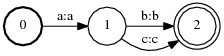
\includegraphics[width=0.5\linewidth]{l.png}
\caption{A word lattice.}
\end{figure}

\column{.5\textwidth}

\begin{figure}
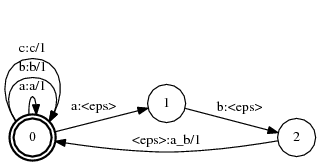
\includegraphics[width=0.6\linewidth]{s.png}
\caption{A segmentation transducer}
\end{figure}

\end{columns}

\begin{figure}
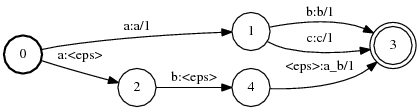
\includegraphics[width=0.8\linewidth]{p.png}
\caption{A phrase lattice produced by composing the word lattice with the segmentation transducer.}
\end{figure}
\end{frame}

% \begin{frame}
% \frametitle{Maximum Spanning Phrases : An example}
% \begin{figure}
% \includegraphics[width=0.8\linewidth]{p_act.png}
% \caption{An actual phrase lattice.}
% \end{figure}
% \end{frame}

\begin{frame}
\frametitle{Maximum spanning phrases}
\begin{block}{Strategy 1 : MSP-greedy (WER = 60.0\% : -2.02\%)}
Select the hypothesis that needs the least number of phrases to cover it (The shortest path in the phrase lattice). 
The word lattice and the phrase segmentation transducer are unweighted in this strategy.
\end{block}

\begin{block}{Strategy 2 : MSP-ASR-draws}
In MSP-greedy if there are draws in length, select the hypothesis that has the best ASR score among the draws. 
The word lattice and the phrase segmentation transducer are unweighted in this strategy.
\end{block}
\end{frame}

\begin{frame}
\begin{block}{Strategy 3 : MSP-Unigram}
Create the phrase lattice (P) by composing weighted ASR lattices with the segmentation transducer(S). Paths in P are weighted 
using the phrase unigram probability.
\begin{align*}
w(\pi_i) = \bigotimes_{p_j \in project(\pi_i)} cost(p_j) \;\; \text{where} \;\; cost(p_j) = \frac{freq(p_j)}{\sum \limits_{k} freq(p_k)}
% w_{\pi_i} = \frac{c(\text{project}(\pi_i))}{\sum_{\pi_j \in \pi}c(\text{project}(\pi_j))}
\end{align*}
where $\pi$ is a path in P and $p_j$ is a phrase in the phrase table.
\end{block}

\begin{block}{Strategy 4 : MSP-Unigram-Length}
To avoid penalizing phrases that are longer and appear less often, scores for paths in S are normalized by the count of phrases with the same length.
\begin{align*}
w(\pi_i) = \bigotimes_{p_j \in project(\pi_i)} cost(p_j) \;\; \text{where} \;\; cost(p_j) = \frac{freq(p_j)}{\sum \limits_{k \; : \; len(p_k) = len(p_j)}freq(p_k)}
% w_{\pi_i} = \frac{c(\text{project}(\pi_i))}{\sum_{\pi_j \in \pi \text{st} len(\pi_j) = len(\pi_i)}c(\text{project}(\pi_j))}
\end{align*}
where $\pi$ is a path in P and $p_j$ is a phrase in the phrase table..
\end{block}
\end{frame}

%------------------------------------------------
\section{SMT strategies and results} % Sections can be created in order to organize your presentation into discrete blocks, all sections and subsections are automatically printed in the table of contents as an overview of the talk
%------------------------------------------------

\begin{frame}
\frametitle{Discussion Forums (DF) decoder baseline results}
Decoding setup :
\begin{itemize} 
\item Evaluated set :  ECA-96 (dev) set.
\item ASR output from Triphone + SAT system.
\item No punctuation in the source and grammar
\item Monotone phrase based model used.
\item All experiments are replicated for seven input types : Human transcripts, ASR 1-best, ASR-Oracle, MSP-{Greedy, ASR-draws, Unigram, Unigram-length}
\end{itemize}

\begin{columns}[c] % The "c" option specifies centered vertical alignment while the "t" option is used for top vertical alignment

\column{.45\textwidth}
\small{
\begin{table}
\begin{center}
\begin{tabular}{|| l || c | c ||}
  \hline 
  \textbf{Input type} & \textbf{R2S} & \textbf{(T-B)/2}\\ \hline
  REF & 0.86 & 25.49\\
  \hline
  ASR 1-best & 0.90 & 39.51\\
  \hline
  ASR-Oracle & 0.89 & 33.50\\
  \hline
\end{tabular}
\caption{Baseline CTS decoding results with the DF SMT system.}
\end{center}
\end{table}
}

\column{.5\textwidth}
\small{
\begin{table}
\begin{center}
\begin{tabular}{|| l || c | c ||}
  \hline 
  \textbf{Input type} & \textbf{R2S} & \textbf{(T-B)/2}\\ \hline
  MSP-greedy & 0.97 & 35.80\\
  \hline
  MSP-ASR-Draws & 0.95 & 36.86\\
  \hline
  MSP-UNI & 0.96 & 36.56\\
  \hline
  MSP-UNI-LEN & 0.94 & 37.36\\
  \hline
\end{tabular}
\caption{Baseline CTS decoding results with the DF SMT system for MSP input.}
\end{center}
\end{table}
}

\end{columns}
\end{frame}


\begin{frame}
\frametitle{Tuning on CTS data}
\begin{itemize}
\item Tuning of the decoding parameters was done on the 97-EVAL-H5 dataset.
\item The hope was to adjust for length (R2S) in the baseline experiment. 
\item Tuning boosted translation model weights and reduced the weights for lm and wc. 
\item Reduction in insertion errors (13667 vs 6186) leads to better decoding (mainly TER) results.
\end{itemize}

\begin{table}
\begin{center}
\begin{tabular}{|| l || c | c || c | c ||}
  \hline 
  {} & \multicolumn{2}{c ||}{\textbf{Baseline}} & \multicolumn{2}{c ||}{\textbf{+Tune-REF}}\\ \hline
  \textbf{Input type} & \textbf{R2S} & \textbf{(T-B)/2} & \textbf{R2S} & \textbf{(T-B)/2}\\ \hline
  REF & 0.86 & 25.49 & 0.97 & 16.42\\
  \hline
  ASR 1-best & 0.90 & 39.51 & 1.05 & 30.75\\
  \hline
  ASR-Oracle & 0.89 & 33.50 & 1.03 & 24.64\\
  \hline
  MSP-greedy & 0.97 & 35.80 & 1.16 & 29.49\\
  \hline
\end{tabular}
\caption{CTS decoding results with tuning on CTS data.}
\end{center}
\end{table}
\end{frame}

\begin{frame}
\frametitle{Tuning the LM interpolation weights}
\begin{itemize}
\item Tuning revealed that a more appropriate interpolation of the weights for the LM components may be needed.
\item Perplexity tuning was done for the LM component interpolation weights using the ECA-supplement dataset
\item Weights increased for the BOLT LM and reduced for everything else.
\end{itemize}

\begin{table}
\begin{center}
\begin{tabular}{|| l || c | c || c | c ||}
  \hline 
  {} & \multicolumn{2}{c ||}{\textbf{+Tune-REF}} & \multicolumn{2}{c ||}{\textbf{+Tune-REF+LM(exp)}}\\ \hline
  \textbf{Input type} & \textbf{R2S} & \textbf{(T-B)/2} & \textbf{R2S} & \textbf{(T-B)/2}\\ \hline
  REF & 0.97 & 16.42 & 0.97 & 16.35\\
  \hline
  ASR 1-best & 1.05 & 30.75 & 1.05 & 30.65\\
  \hline
  ASR-Oracle & 1.03 & 24.64 & 1.02 & 24.52\\
  \hline
  MSP-greedy & 1.16 & 29.49 & 1.16 & 29.39\\
  \hline
\end{tabular}
\caption{CTS decoding results, tuned on CTS data, tuned LM weights}
\end{center}
\end{table}
\end{frame}

% \begin{frame}
% \frametitle{Hesitations, noise and non-vocal markers in tuning data}
% \begin{itemize}
% \item Informal speech contains hesitations, laughter, noise and other disfluencies and non-vocal sounds.
% \item Even though these are produced by the ASR, they are typically stripped off before translation.
% \item Utterances that only contained these symbols are now empty. 
% \item Tuning without these empty sentences yields better R2S on decoding but worse $(T-B)/2$ results. 
% \end{itemize}

% \begin{table}
% \begin{center}
% \begin{tabular}{|| c || c | c || c | c ||}
%   \hline 
%   {} & \multicolumn{2}{c ||}{+Tune-REF+LM(exp)} & \multicolumn{2}{c ||}{- empty-sent}\\ \hline
%   \textbf{Input type} & \textbf{R2S} & \textbf{(T-B)/2} & \textbf{R2S} & \textbf{(T-B)/2}\\ \hline
%   REF & 0.97 & 16.35 & 0.96 & 17.36\\
%   \hline
%   ASR 1-best & 1.05 & 30.65 & 1.03 & 31.37\\
%   \hline
%   MSP-greedy & 1.16 & 29.39 & 1.13 & 29.76\\
%   \hline
%   ASR-Oracle & 1.02 & 24.52 & 1.00 & 25.17 \\
%   \hline
%   MSP-ASR-Draws & 1.12 & 29.55 & 1.09 & 30.10\\
%   \hline
%   MSP-UNI & 1.14 & 29.69 & 1.11 & 30.12\\
%   \hline
%   MSP-UNI-LEN & 1.11 & 29.91 & 1.09 & 30.40\\
%   \hline
% \end{tabular}
% \caption{CTS decoding results, tuned on non-empty CTS data, tuned LM weights}
% \end{center}
% \end{table}
% \end{frame}

\begin{frame}
\frametitle{Tuning on ASR output}
\begin{itemize}
\item Tuned on ASR 1-best output for 97-H5-eval.
\item Decoding yields best R2S but worse ($\sim$ 1.8 points) (T-B)/2 results. 
\item Tuning set significantly smaller because of the large number of empty sentences.
\item Tuning on high WER may cause this, results may change with lower WER ASR output.
\end{itemize}

\begin{table}
\begin{center}
\begin{tabular}{|| l || c | c || c | c ||}
  \hline 
  {} & \multicolumn{2}{c ||}{\textbf{+Tune-REF+LM(exp)}} & \multicolumn{2}{c ||}{\textbf{+Tune-ASR+LM(exp)}}\\ \hline
  \textbf{Input type} & \textbf{R2S} & \textbf{(T-B)/2} & \textbf{R2S} & \textbf{(T-B)/2}\\ \hline
  REF & 0.97 & 16.35 & 0.95 & 18.17\\
  \hline
  ASR 1-best & 1.05 & 30.65 & 1.02 & 31.96\\
  \hline
  ASR-Oracle & 1.02 & 24.52 & 0.99 & 25.86\\
  \hline
  MSP-greedy & 1.16 & 29.39 & 1.11 & 30.00\\
  \hline
\end{tabular}
\caption{CTS decoding results, tuned on non-empty ASR output, tuned LM weights}
\end{center}
\end{table}
\end{frame}

% \begin{frame}
% \frametitle{Length constrained tuning}
% Describe strategy of tuning on smaller datasets for smaller datasets and the same for the larger. Use the next slide to include results in the
% form of a matrix. Decide on the structure.
% \end{frame}

\begin{frame}
\frametitle{A hope for the future : Decoding ASR output with lower WERs}
Decoding ASR output with a lower WER results in a significant gain in (T-B)/2 scores.

\begin{table}
\begin{center}
\begin{tabular}{| l | c | c || c |}
  \hline 
  \textbf{ASR-model} & \textbf{WER} & \textbf{R2S} & \textbf{(T-B)/2}\\ \hline
  Triphone+SAT & 57.98\% & 0.95 & 30.65\\
  \hline
  +SGMM 1-best & 52.74\% & 0.95 & 28.55\\
  \hline
  +DNN & 51.80\% & 0.96 & 28.58\\
  \hline
\end{tabular}
\caption{CTS decoding results for the ASR 1-best from three different ASR models with varying WER. The SMT system parameters and the LM weights are tuned on CTS data}
\end{center}
\end{table} 
\end{frame}

% %------------------------------------------------
% \section{Speech Translation Errors} % Sections can be created in order to organize your presentation into discrete blocks, all sections and subsections are automatically printed in the table of contents as an overview of the talk
% %------------------------------------------------
% \begin{frame}
% \frametitle{Most common errors}
% n-gram coverage ? Most severe mis-recognitions? How do you measure this? Put this if you have time.
% \end{frame}

\begin{frame}
\frametitle{Backchanneling}
\begin{columns}[c] % The "c" option specifies centered vertical alignment while the "t" option is used for top vertical alignment

\column{.45\textwidth} % Left column and width
\vspace{-10mm}
\begin{itemize}
\item The ASR system frequently mis-recognizes very short utterances with hesitations/non-vocal markers.
\item These mis-recognitions are typically utterances produced by back-channeling.
\item Hence the ASR output after stripping these is much shorter (1027 additional empty segments)
\end{itemize}
\column{.5\textwidth}
\begin{table}
\begin{center}
\begin{tabular}{| l | c |}
\hline
\textbf{Utterance} & \textbf{Frequency}\\ \hline
yes & 476\\
m & 131\\
mm & 72\\
what & 39\\
yes yes & 29\\
ha & 19\\
ok & 18\\
umm & 13\\
na & 8\\
aha & 7\\
m m & 6\\
yes yes yes & 4\\
\hline
\end{tabular}
\caption{Frequent utterances mis-recognized by the ASR for hesitation/non-vocal sounds}
\end{center}
\end{table} 
\end{columns}
\end{frame}

%------------------------------------------------
\section{Conclusion} % Sections can be created in order to organize your presentation into discrete blocks, all sections and subsections are automatically printed in the table of contents as an overview of the talk
%------------------------------------------------

\begin{frame}
\frametitle{Conclusions}
\begin{itemize}
\item The \textbf{high WER} of the ASR output makes this a hard problem to tackle.
\item The difference in WERs and decoding results between the ASR 1-best and the \textbf{ASR-oracle} is significant.
\item Better methods of selecting hypotheses from ASR lattices are needed. \textbf{1.26 $(T-B)/2$} point improvement over the ASR 1-best with MSP strategies.
\item Better decoding results may arise from paths in the ASR lattices that have worse WER. 
\item \textbf{9 $(T-B)/2$} point improvement with tuning model parameters and training weights for LM components.
\item Cumulative gain of \textbf{10 $(T-B)/2$} points over the baseline DF results
\end{itemize}
\end{frame}

\begin{frame}
\frametitle{Future work}
\begin{itemize}
\item Validate results on ASR output with lower WER.
\item Combined tuning on ASR output and human transcripts.
\item Include CTS data in the TM and LM for SMT
\item \textbf{Multiple training source streams : Most common mis-recognitions from the ASR can be added to the SMT phrase table. This should help correct these common mistakes.}
\item \textbf{Apply the concept of selecting hypotheses from the lattice (MSP) in Hiero based translation.}
\end{itemize}
\end{frame}

\begin{frame}
\Huge{\centerline{Questions?}}
\end{frame}

%----------------------------------------------------------------------------------------

\end{document} 
